\documentclass[a4paper]{book}
\usepackage{a4wide}
\usepackage{makeidx}
\usepackage{graphicx}
\usepackage{multicol}
\usepackage{float}
\usepackage{listings}
\usepackage{color}
\usepackage{textcomp}
\usepackage{alltt}
\usepackage{times}
\usepackage{ifpdf}
\ifpdf
\usepackage[pdftex,
            pagebackref=true,
            colorlinks=true,
            linkcolor=blue,
            unicode
           ]{hyperref}
\else
\usepackage[ps2pdf,
            pagebackref=true,
            colorlinks=true,
            linkcolor=blue,
            unicode
           ]{hyperref}
\usepackage{pspicture}
\fi
\usepackage[utf8]{inputenc}
\usepackage{doxygen}
\lstset{language=C++,inputencoding=utf8,basicstyle=\footnotesize,breaklines=true,breakatwhitespace=true,tabsize=8,numbers=left }
\makeindex
\setcounter{tocdepth}{3}
\renewcommand{\footrulewidth}{0.4pt}
\begin{document}
\hypersetup{pageanchor=false}
\begin{titlepage}
\vspace*{7cm}
\begin{center}
{\Large Reference Manual}\\
\vspace*{1cm}
{\large Generated by Doxygen 1.7.1}\\
\vspace*{0.5cm}
{\small Tue Mar 27 2012 02:59:18}\\
\end{center}
\end{titlepage}
\clearemptydoublepage
\pagenumbering{roman}
\tableofcontents
\clearemptydoublepage
\pagenumbering{arabic}
\hypersetup{pageanchor=true}
\chapter{Class Index}
\section{Class List}
Here are the classes, structs, unions and interfaces with brief descriptions:\begin{DoxyCompactList}
\item\contentsline{section}{\hyperlink{classBooleanExpression}{BooleanExpression} }{\pageref{classBooleanExpression}}{}
\item\contentsline{section}{\hyperlink{classMaze}{Maze} }{\pageref{classMaze}}{}
\item\contentsline{section}{\hyperlink{classNimGameConf}{NimGameConf} }{\pageref{classNimGameConf}}{}
\item\contentsline{section}{\hyperlink{classRebus}{Rebus} }{\pageref{classRebus}}{}
\item\contentsline{section}{\hyperlink{classSudokuBoard}{SudokuBoard} }{\pageref{classSudokuBoard}}{}
\item\contentsline{section}{\hyperlink{classXOBoard}{XOBoard} }{\pageref{classXOBoard}}{}
\item\contentsline{section}{\hyperlink{classXOGame}{XOGame} }{\pageref{classXOGame}}{}
\end{DoxyCompactList}

\chapter{Class Documentation}
\hypertarget{classBooleanExpression}{
\section{BooleanExpression Class Reference}
\label{classBooleanExpression}\index{BooleanExpression@{BooleanExpression}}
}
\subsection*{Public Member Functions}
\begin{DoxyCompactItemize}
\item 
\hypertarget{classBooleanExpression_add76e02bf45058445aaf70fd6400108c}{
boolean {\bfseries isValid} ()}
\label{classBooleanExpression_add76e02bf45058445aaf70fd6400108c}

\item 
\hypertarget{classBooleanExpression_ae02cb61914b378cdd28cd858d9e8a4a0}{
Lexem\mbox{[}$\,$\mbox{]} {\bfseries getLexems} ()}
\label{classBooleanExpression_ae02cb61914b378cdd28cd858d9e8a4a0}

\end{DoxyCompactItemize}
\subsection*{Package Functions}
\begin{DoxyCompactItemize}
\item 
\hypertarget{classBooleanExpression_a0ac4c6f0eb4d1e9b96bd837aa31de159}{
{\bfseries BooleanExpression} (String stringRepresentation)}
\label{classBooleanExpression_a0ac4c6f0eb4d1e9b96bd837aa31de159}

\end{DoxyCompactItemize}


The documentation for this class was generated from the following file:\begin{DoxyCompactItemize}
\item 
/home/marcvs/Desktop/working/pa-\/materiale/pa/codeBase/Java/src/BooleanExpression.java\end{DoxyCompactItemize}

\hypertarget{classMaze}{
\section{Maze Class Reference}
\label{classMaze}\index{Maze@{Maze}}
}
Inheritance diagram for Maze:\begin{figure}[H]
\begin{center}
\leavevmode
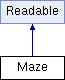
\includegraphics[height=2.000000cm]{classMaze}
\end{center}
\end{figure}
\subsection*{Public Member Functions}
\begin{DoxyCompactItemize}
\item 
\hypertarget{classMaze_a8f1cc7d8dd3fa426ace16bf32f54f24f}{
{\bfseries Maze} (int height, int width)}
\label{classMaze_a8f1cc7d8dd3fa426ace16bf32f54f24f}

\item 
\hypertarget{classMaze_a3f9b79edb99a9726da62bc6823ea9149}{
int {\bfseries get\_\-width} ()}
\label{classMaze_a3f9b79edb99a9726da62bc6823ea9149}

\item 
\hypertarget{classMaze_a43a3408e506b2f2463fc985865b3c850}{
int {\bfseries get\_\-height} ()}
\label{classMaze_a43a3408e506b2f2463fc985865b3c850}

\item 
\hypertarget{classMaze_a18724de009238efe119be4c80906416f}{
boolean {\bfseries is\_\-walkable} (int line, int column)}
\label{classMaze_a18724de009238efe119be4c80906416f}

\item 
\hypertarget{classMaze_a1156760e57f75cd36241a9244f902277}{
boolean {\bfseries is\_\-walkable} (\hyperlink{classCoord}{Coord} coord)}
\label{classMaze_a1156760e57f75cd36241a9244f902277}

\item 
\hypertarget{classMaze_ac223c8189bee28e047d4399cff5fa765}{
boolean {\bfseries is\_\-exit\_\-point} (int line, int column)}
\label{classMaze_ac223c8189bee28e047d4399cff5fa765}

\item 
\hypertarget{classMaze_a5ee98f5633093dc2e1cba6c03e4ddb54}{
boolean {\bfseries is\_\-exit\_\-point} (\hyperlink{classCoord}{Coord} coord)}
\label{classMaze_a5ee98f5633093dc2e1cba6c03e4ddb54}

\item 
\hypertarget{classMaze_a258ccfd950d62359774ed00a75591eaa}{
void {\bfseries mark\_\-solution\_\-step} (int line, int column)}
\label{classMaze_a258ccfd950d62359774ed00a75591eaa}

\item 
\hypertarget{classMaze_a0b27a912b886cd33a45d53789e4f2f1b}{
void {\bfseries mark\_\-solution\_\-step} (\hyperlink{classCoord}{Coord} coord)}
\label{classMaze_a0b27a912b886cd33a45d53789e4f2f1b}

\item 
\hypertarget{classMaze_a70725da73e2032a640bd80db1a51b1dc}{
void {\bfseries read} (Scanner scanner)}
\label{classMaze_a70725da73e2032a640bd80db1a51b1dc}

\item 
\hypertarget{classMaze_a6eb47c884e545475598f784707088f8b}{
void {\bfseries print} ()}
\label{classMaze_a6eb47c884e545475598f784707088f8b}

\end{DoxyCompactItemize}


The documentation for this class was generated from the following file:\begin{DoxyCompactItemize}
\item 
/home/marcvs/Desktop/working/pa-\/materiale/pa/codeBase/Java/src/Maze.java\end{DoxyCompactItemize}

\hypertarget{classNimGameConf}{
\section{NimGameConf Class Reference}
\label{classNimGameConf}\index{NimGameConf@{NimGameConf}}
}
\subsection*{Public Member Functions}
\begin{DoxyCompactItemize}
\item 
\hypertarget{classNimGameConf_aca38313f09d82be07a32770a9f6875cc}{
{\bfseries NimGameConf} (int n)}
\label{classNimGameConf_aca38313f09d82be07a32770a9f6875cc}

\item 
size\_\-t \hyperlink{classNimGameConf_a6562b1e5b81ef42b350abdb7b3f024be}{size} ()
\begin{DoxyCompactList}\small\item\em Functie care intoarce dimensiunea celei mai mari gramezi din joc. \item\end{DoxyCompactList}\item 
bool \hyperlink{classNimGameConf_a9d882cf631a20956c0e542dd71a8b726}{gameOver} ()
\begin{DoxyCompactList}\small\item\em Functie care spune daca jocul s-\/a terminat. Jocul se termina atunci cand nu mai exista nici o gramada cu cel putin trei pietricele. \item\end{DoxyCompactList}\item 
\hypertarget{classNimGameConf_ad8c71ec49bf1a773c169f6a57523309e}{
int \& \hyperlink{classNimGameConf_ad8c71ec49bf1a773c169f6a57523309e}{operator\mbox{[}$\,$\mbox{]}} (const unsigned int index)}
\label{classNimGameConf_ad8c71ec49bf1a773c169f6a57523309e}

\begin{DoxyCompactList}\small\item\em Operator care permite accesul la orice gramada din joc. \item\end{DoxyCompactList}\item 
void \hyperlink{classNimGameConf_ad19bf383bbd4eafc893491e31059d777}{split} (int heap, int a, int b)
\begin{DoxyCompactList}\small\item\em Functie care imparte o gramada in alte doua gramezi mai mici. \item\end{DoxyCompactList}\item 
\hypertarget{classNimGameConf_a8001a96febdfe2ce67ae8cee025a89e0}{
void \hyperlink{classNimGameConf_a8001a96febdfe2ce67ae8cee025a89e0}{unsplit} (int heap, int a, int b)}
\label{classNimGameConf_a8001a96febdfe2ce67ae8cee025a89e0}

\begin{DoxyCompactList}\small\item\em Inversul functiei split. Reasambleaza doua gramezi in gramada originala. Nu este o miscare valida de gameplay, dar poate fi utila la expandarea arborelui. \item\end{DoxyCompactList}\end{DoxyCompactItemize}
\subsection*{Friends}
\begin{DoxyCompactItemize}
\item 
\hypertarget{classNimGameConf_a119d80a72d6c9f144fc19036dabc1827}{
std::ostream \& {\bfseries operator$<$$<$} (std::ostream \&, const \hyperlink{classNimGameConf}{NimGameConf} \&)}
\label{classNimGameConf_a119d80a72d6c9f144fc19036dabc1827}

\end{DoxyCompactItemize}


\subsection{Member Function Documentation}
\hypertarget{classNimGameConf_a9d882cf631a20956c0e542dd71a8b726}{
\index{NimGameConf@{NimGameConf}!gameOver@{gameOver}}
\index{gameOver@{gameOver}!NimGameConf@{NimGameConf}}
\subsubsection[{gameOver}]{\setlength{\rightskip}{0pt plus 5cm}bool NimGameConf::gameOver (
\begin{DoxyParamCaption}
{}
\end{DoxyParamCaption}
)\hspace{0.3cm}{\ttfamily  \mbox{[}inline\mbox{]}}}}
\label{classNimGameConf_a9d882cf631a20956c0e542dd71a8b726}


Functie care spune daca jocul s-\/a terminat. Jocul se termina atunci cand nu mai exista nici o gramada cu cel putin trei pietricele. 

\begin{DoxyReturn}{Returns}
{\bfseries true} daca jocul s-\/a terminat, sau {\bfseries false} altfel. 
\end{DoxyReturn}
\hypertarget{classNimGameConf_a6562b1e5b81ef42b350abdb7b3f024be}{
\index{NimGameConf@{NimGameConf}!size@{size}}
\index{size@{size}!NimGameConf@{NimGameConf}}
\subsubsection[{size}]{\setlength{\rightskip}{0pt plus 5cm}size\_\-t NimGameConf::size (
\begin{DoxyParamCaption}
{}
\end{DoxyParamCaption}
)\hspace{0.3cm}{\ttfamily  \mbox{[}inline\mbox{]}}}}
\label{classNimGameConf_a6562b1e5b81ef42b350abdb7b3f024be}


Functie care intoarce dimensiunea celei mai mari gramezi din joc. 

\begin{DoxyReturn}{Returns}
Dimensiunea celei mai mari gramezi din joc (cea initiala). 
\end{DoxyReturn}
\hypertarget{classNimGameConf_ad19bf383bbd4eafc893491e31059d777}{
\index{NimGameConf@{NimGameConf}!split@{split}}
\index{split@{split}!NimGameConf@{NimGameConf}}
\subsubsection[{split}]{\setlength{\rightskip}{0pt plus 5cm}void NimGameConf::split (
\begin{DoxyParamCaption}
\item[{int}]{ heap, }
\item[{int}]{ a, }
\item[{int}]{ b}
\end{DoxyParamCaption}
)\hspace{0.3cm}{\ttfamily  \mbox{[}inline\mbox{]}}}}
\label{classNimGameConf_ad19bf383bbd4eafc893491e31059d777}


Functie care imparte o gramada in alte doua gramezi mai mici. 


\begin{DoxyParams}{Parameters}
\item[{\em heap}]Gramada ce trebuie impartita. \item[{\em a}]Dimensiunea primei gramezi. \item[{\em b}]Dimensiunea celei de-\/a doua gramezi. \end{DoxyParams}


The documentation for this class was generated from the following file:\begin{DoxyCompactItemize}
\item 
/home/marcvs/Desktop/working/pa-\/materiale/pa/codeBase/C++/include/Nim.h\end{DoxyCompactItemize}

\hypertarget{classRebus}{
\section{Rebus Class Reference}
\label{classRebus}\index{Rebus@{Rebus}}
}
Inheritance diagram for Rebus:\begin{figure}[H]
\begin{center}
\leavevmode
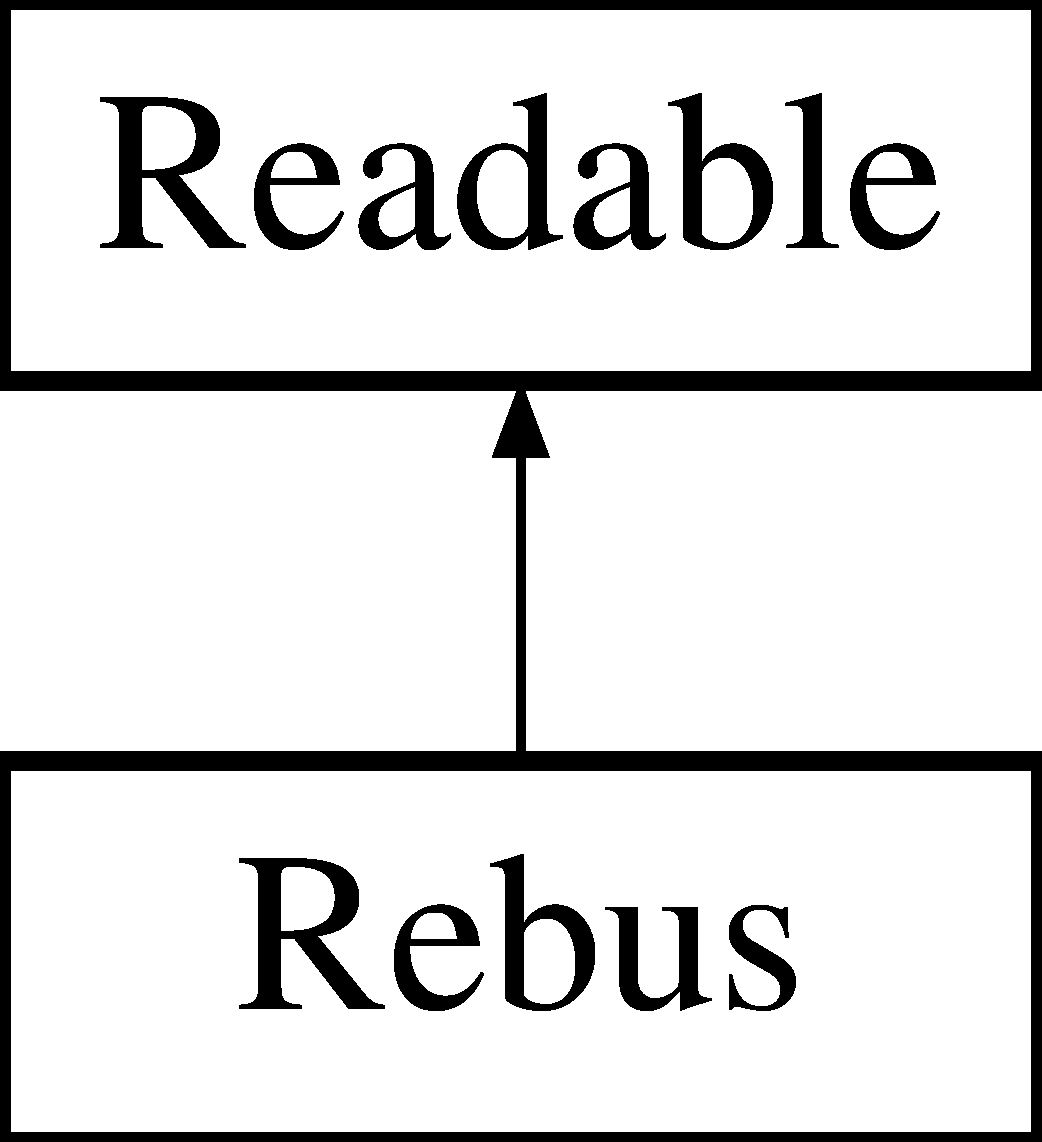
\includegraphics[height=2.000000cm]{classRebus}
\end{center}
\end{figure}
\subsection*{Public Member Functions}
\begin{DoxyCompactItemize}
\item 
\hypertarget{classRebus_a2495b8ab66b8b5fc73be661e6ccb85d3}{
char {\bfseries get} (int row, int column)}
\label{classRebus_a2495b8ab66b8b5fc73be661e6ccb85d3}

\item 
\hypertarget{classRebus_a33c68ead613e1cad7e1e274451f769c0}{
void {\bfseries put} (int row, int column, char c)}
\label{classRebus_a33c68ead613e1cad7e1e274451f769c0}

\item 
\hypertarget{classRebus_ab1ffa625317a5f6f05c75ec072a4bf53}{
void {\bfseries read} (Scanner scanner)}
\label{classRebus_ab1ffa625317a5f6f05c75ec072a4bf53}

\item 
\hypertarget{classRebus_ad208ddcbae9a498c5e8ef2beec2a3306}{
String {\bfseries toString} ()}
\label{classRebus_ad208ddcbae9a498c5e8ef2beec2a3306}

\end{DoxyCompactItemize}
\subsection*{Public Attributes}
\begin{DoxyCompactItemize}
\item 
\hypertarget{classRebus_a0d21b9515af691a04c515a3c163bd683}{
int {\bfseries rows}}
\label{classRebus_a0d21b9515af691a04c515a3c163bd683}

\item 
\hypertarget{classRebus_a71ec10584853e625028ea0c7c4932256}{
int {\bfseries columns}}
\label{classRebus_a71ec10584853e625028ea0c7c4932256}

\end{DoxyCompactItemize}
\subsection*{Package Functions}
\begin{DoxyCompactItemize}
\item 
\hypertarget{classRebus_ae7febf865939cb84fc08a087d12ee465}{
void {\bfseries putString} (int row, int column, String s)}
\label{classRebus_ae7febf865939cb84fc08a087d12ee465}

\item 
\hypertarget{classRebus_a7f568be5d10645247a9c3b9c3aefd31b}{
void {\bfseries eraseString} (int row, int column)}
\label{classRebus_a7f568be5d10645247a9c3b9c3aefd31b}

\item 
\hypertarget{classRebus_a51b184a4ff31ffb8d696daf86b6027f9}{
void {\bfseries erase} (int row, int column)}
\label{classRebus_a51b184a4ff31ffb8d696daf86b6027f9}

\item 
\hypertarget{classRebus_ad429f688c0bd500988843f21426bca97}{
boolean {\bfseries is\_\-empty} (int row, int column)}
\label{classRebus_ad429f688c0bd500988843f21426bca97}

\item 
\hypertarget{classRebus_a75a4903e5f1d6ecb72c3689fda4422f3}{
boolean {\bfseries is\_\-done} ()}
\label{classRebus_a75a4903e5f1d6ecb72c3689fda4422f3}

\end{DoxyCompactItemize}
\subsection*{Package Attributes}
\begin{DoxyCompactItemize}
\item 
\hypertarget{classRebus_aa874c93e563860b32ee8d70bd15b66c7}{
char\mbox{[}$\,$\mbox{]}\mbox{[}$\,$\mbox{]} {\bfseries m}}
\label{classRebus_aa874c93e563860b32ee8d70bd15b66c7}

\item 
\hypertarget{classRebus_a3279788d9a6d47b8c7bc6857582d298c}{
char\mbox{[}$\,$\mbox{]}\mbox{[}$\,$\mbox{]} {\bfseries ref}}
\label{classRebus_a3279788d9a6d47b8c7bc6857582d298c}

\end{DoxyCompactItemize}


The documentation for this class was generated from the following file:\begin{DoxyCompactItemize}
\item 
/home/marcvs/Desktop/working/pa-\/materiale/pa/codeBase/Java/src/Rebus.java\end{DoxyCompactItemize}

\hypertarget{classSudokuBoard}{
\section{SudokuBoard Class Reference}
\label{classSudokuBoard}\index{SudokuBoard@{SudokuBoard}}
}
\subsection*{Classes}
\begin{DoxyCompactItemize}
\item 
class {\bfseries BitSet}
\end{DoxyCompactItemize}
\subsection*{Public Member Functions}
\begin{DoxyCompactItemize}
\item 
bool \hyperlink{classSudokuBoard_aa5d810273b58996f5eb00522dc04c012}{impossible} (int row, int col)
\begin{DoxyCompactList}\small\item\em Functie care spune daca pentru linia {\bfseries row} si coloana {\bfseries col} din careu nu mai avem nici o posibilitate de completare. \item\end{DoxyCompactList}\item 
int \hyperlink{classSudokuBoard_add88bcf66d345b2822335d92713b8714}{unique\_\-possibility} (int row, int col)
\begin{DoxyCompactList}\small\item\em Functie care verifica daca nu cumva pentru linia {\bfseries row} si coloana {\bfseries col} nu exista decat o singura metoda de completare. \item\end{DoxyCompactList}\item 
bool \hyperlink{classSudokuBoard_a4ae4146f3ebed70288b41adb9ee1d8ed}{allows} (int row, int col, int i)
\begin{DoxyCompactList}\small\item\em Functie care verifica daca este posibil sa se completeze valoarea {\bfseries i} la celula de coordonate {\bfseries row}, {\bfseries col} \item\end{DoxyCompactList}\item 
void \hyperlink{classSudokuBoard_aff759e2337f20e107ed7e70d5cd8ca41}{put} (int row, int col, int i)
\begin{DoxyCompactList}\small\item\em Functie care completeaza o valoare intr-\/o celula din careu. {\bfseries ATENTIE!} Este responsabilitatea voastra sa va asigurati ca nu suprascrieti o valoare deja pusa acolo! \item\end{DoxyCompactList}\item 
bool \hyperlink{classSudokuBoard_a1e4d6cac572c9f4d4a573265da99f517}{is\_\-empty} (int row, int col)
\begin{DoxyCompactList}\small\item\em Functie care verifica daca o celula din careu nu a fost completata. \item\end{DoxyCompactList}\item 
bool \hyperlink{classSudokuBoard_ad53cca0148ad57fdaa05f9b92000fe66}{is\_\-done} ()
\begin{DoxyCompactList}\small\item\em Functie care verifica daca un careu s-\/a terminat de completat. \item\end{DoxyCompactList}\end{DoxyCompactItemize}
\subsection*{Friends}
\begin{DoxyCompactItemize}
\item 
\hypertarget{classSudokuBoard_ac31711643f4d24c0e0e312d763a37d62}{
std::ostream \& \hyperlink{classSudokuBoard_ac31711643f4d24c0e0e312d763a37d62}{operator$<$$<$} (std::ostream \&out, \hyperlink{classSudokuBoard}{SudokuBoard} \&right)}
\label{classSudokuBoard_ac31711643f4d24c0e0e312d763a37d62}

\begin{DoxyCompactList}\small\item\em Operator care scrie o grila de Sudoku intr-\/un stream de iesire. \item\end{DoxyCompactList}\end{DoxyCompactItemize}


\subsection{Member Function Documentation}
\hypertarget{classSudokuBoard_a4ae4146f3ebed70288b41adb9ee1d8ed}{
\index{SudokuBoard@{SudokuBoard}!allows@{allows}}
\index{allows@{allows}!SudokuBoard@{SudokuBoard}}
\subsubsection[{allows}]{\setlength{\rightskip}{0pt plus 5cm}bool SudokuBoard::allows (
\begin{DoxyParamCaption}
\item[{int}]{ row, }
\item[{int}]{ col, }
\item[{int}]{ i}
\end{DoxyParamCaption}
)\hspace{0.3cm}{\ttfamily  \mbox{[}inline\mbox{]}}}}
\label{classSudokuBoard_a4ae4146f3ebed70288b41adb9ee1d8ed}


Functie care verifica daca este posibil sa se completeze valoarea {\bfseries i} la celula de coordonate {\bfseries row}, {\bfseries col} 


\begin{DoxyParams}{Parameters}
\item[{\em row}]Linia pentru care verificam \item[{\em col}]Coloana pentru care verificam \item[{\em i}]Valoarea despre care intrebam daca este permisibila \end{DoxyParams}
\begin{DoxyReturn}{Returns}
Functia intoarce {\bfseries true} daca completarea este corecta. 
\end{DoxyReturn}
\hypertarget{classSudokuBoard_aa5d810273b58996f5eb00522dc04c012}{
\index{SudokuBoard@{SudokuBoard}!impossible@{impossible}}
\index{impossible@{impossible}!SudokuBoard@{SudokuBoard}}
\subsubsection[{impossible}]{\setlength{\rightskip}{0pt plus 5cm}bool SudokuBoard::impossible (
\begin{DoxyParamCaption}
\item[{int}]{ row, }
\item[{int}]{ col}
\end{DoxyParamCaption}
)\hspace{0.3cm}{\ttfamily  \mbox{[}inline\mbox{]}}}}
\label{classSudokuBoard_aa5d810273b58996f5eb00522dc04c012}


Functie care spune daca pentru linia {\bfseries row} si coloana {\bfseries col} din careu nu mai avem nici o posibilitate de completare. 


\begin{DoxyParams}{Parameters}
\item[{\em row}]Linia pentru care verificam \item[{\em col}]Coloana pentru care verificam \end{DoxyParams}
\begin{DoxyReturn}{Returns}
Functia intoarce {\bfseries true} daca este imposibil sa mai completezi celula de coordonate (row,col) 
\end{DoxyReturn}
\hypertarget{classSudokuBoard_ad53cca0148ad57fdaa05f9b92000fe66}{
\index{SudokuBoard@{SudokuBoard}!is\_\-done@{is\_\-done}}
\index{is\_\-done@{is\_\-done}!SudokuBoard@{SudokuBoard}}
\subsubsection[{is\_\-done}]{\setlength{\rightskip}{0pt plus 5cm}bool SudokuBoard::is\_\-done (
\begin{DoxyParamCaption}
{}
\end{DoxyParamCaption}
)\hspace{0.3cm}{\ttfamily  \mbox{[}inline\mbox{]}}}}
\label{classSudokuBoard_ad53cca0148ad57fdaa05f9b92000fe66}


Functie care verifica daca un careu s-\/a terminat de completat. 

\begin{DoxyReturn}{Returns}
Functia intoarce {\bfseries true} daca s-\/a terminat completarea careului. 
\end{DoxyReturn}
\hypertarget{classSudokuBoard_a1e4d6cac572c9f4d4a573265da99f517}{
\index{SudokuBoard@{SudokuBoard}!is\_\-empty@{is\_\-empty}}
\index{is\_\-empty@{is\_\-empty}!SudokuBoard@{SudokuBoard}}
\subsubsection[{is\_\-empty}]{\setlength{\rightskip}{0pt plus 5cm}bool SudokuBoard::is\_\-empty (
\begin{DoxyParamCaption}
\item[{int}]{ row, }
\item[{int}]{ col}
\end{DoxyParamCaption}
)\hspace{0.3cm}{\ttfamily  \mbox{[}inline\mbox{]}}}}
\label{classSudokuBoard_a1e4d6cac572c9f4d4a573265da99f517}


Functie care verifica daca o celula din careu nu a fost completata. 

\begin{DoxyReturn}{Returns}
Functia intoarce {\bfseries true} daca celula respectiva este libera si {\bfseries false} altfel. 
\end{DoxyReturn}
\hypertarget{classSudokuBoard_aff759e2337f20e107ed7e70d5cd8ca41}{
\index{SudokuBoard@{SudokuBoard}!put@{put}}
\index{put@{put}!SudokuBoard@{SudokuBoard}}
\subsubsection[{put}]{\setlength{\rightskip}{0pt plus 5cm}void SudokuBoard::put (
\begin{DoxyParamCaption}
\item[{int}]{ row, }
\item[{int}]{ col, }
\item[{int}]{ i}
\end{DoxyParamCaption}
)\hspace{0.3cm}{\ttfamily  \mbox{[}inline\mbox{]}}}}
\label{classSudokuBoard_aff759e2337f20e107ed7e70d5cd8ca41}


Functie care completeaza o valoare intr-\/o celula din careu. {\bfseries ATENTIE!} Este responsabilitatea voastra sa va asigurati ca nu suprascrieti o valoare deja pusa acolo! 


\begin{DoxyParams}{Parameters}
\item[{\em row}]Linia pentru care verificam \item[{\em col}]Coloana pentru care verificam \item[{\em i}]Valoarea pe care dorim sa o trecem in celula \end{DoxyParams}
\hypertarget{classSudokuBoard_add88bcf66d345b2822335d92713b8714}{
\index{SudokuBoard@{SudokuBoard}!unique\_\-possibility@{unique\_\-possibility}}
\index{unique\_\-possibility@{unique\_\-possibility}!SudokuBoard@{SudokuBoard}}
\subsubsection[{unique\_\-possibility}]{\setlength{\rightskip}{0pt plus 5cm}int SudokuBoard::unique\_\-possibility (
\begin{DoxyParamCaption}
\item[{int}]{ row, }
\item[{int}]{ col}
\end{DoxyParamCaption}
)\hspace{0.3cm}{\ttfamily  \mbox{[}inline\mbox{]}}}}
\label{classSudokuBoard_add88bcf66d345b2822335d92713b8714}


Functie care verifica daca nu cumva pentru linia {\bfseries row} si coloana {\bfseries col} nu exista decat o singura metoda de completare. 


\begin{DoxyParams}{Parameters}
\item[{\em row}]Linia pentru care verificam \item[{\em col}]Coloana pentru care verificam \end{DoxyParams}
\begin{DoxyReturn}{Returns}
Functia intoarce o cifra nenula intre 1 si 9 daca exista o singura varianta de completare, si 0 daca exista mai multe variante sau nici o varianta. 
\end{DoxyReturn}


The documentation for this class was generated from the following files:\begin{DoxyCompactItemize}
\item 
/home/marcvs/Desktop/working/pa-\/materiale/pa/codeBase/C++/include/SudokuBoard.h\item 
/home/marcvs/Desktop/working/pa-\/materiale/pa/codeBase/C++/src/SudokuBoard.cpp\end{DoxyCompactItemize}

\hypertarget{classXOBoard}{
\section{XOBoard Class Reference}
\label{classXOBoard}\index{XOBoard@{XOBoard}}
}
\subsection*{Public Types}
\begin{DoxyCompactItemize}
\item 
enum {\bfseries Player} \{ {\bfseries PlayerX}, 
{\bfseries PlayerO}
 \}
\end{DoxyCompactItemize}
\subsection*{Public Member Functions}
\begin{DoxyCompactItemize}
\item 
\hypertarget{classXOBoard_a5740df9f6637e64adb7745228820b608}{
\hyperlink{classXOBoard_a5740df9f6637e64adb7745228820b608}{XOBoard} ()}
\label{classXOBoard_a5740df9f6637e64adb7745228820b608}

\begin{DoxyCompactList}\small\item\em Constructor fara parametri care instantiaza o tabla goala pe care nu este marcat nimic. \item\end{DoxyCompactList}\item 
bool \hyperlink{classXOBoard_afc284df051b707b824bc8289e5bffd22}{is\_\-empty} (int x, int y) const 
\begin{DoxyCompactList}\small\item\em Metoda care verifica daca o celula este libera sau nu. \item\end{DoxyCompactList}\item 
char \hyperlink{classXOBoard_a850b7cbdb93c080eb7db8d749bf1aafa}{get} (int x, int y) const 
\begin{DoxyCompactList}\small\item\em Metoda care intoarce caracterul de pe tabla. \item\end{DoxyCompactList}\item 
void \hyperlink{classXOBoard_a3190b1cd4b6d1665bb0b6c35411d0c3e}{put} (Player player, int x, int y)
\begin{DoxyCompactList}\small\item\em Metoda care bifeaza o celula de pe tabla in numele unui jucator. \item\end{DoxyCompactList}\item 
void \hyperlink{classXOBoard_a6e72af673a48b7a4de79d7b738a690c1}{erase} (int x, int y)
\begin{DoxyCompactList}\small\item\em Metoda care sterge valoarea dintr-\/o celula de pe tabla. \item\end{DoxyCompactList}\item 
bool \hyperlink{classXOBoard_a58b290b18786b246c9051958819b1d4f}{is\_\-full} () const 
\begin{DoxyCompactList}\small\item\em Metoda care spune daca tabla s-\/a terminat de completat sau nu. \item\end{DoxyCompactList}\item 
int \hyperlink{classXOBoard_a8affd589eb32be52b4a58cdb487eaee5}{get\_\-score} (Player player) const 
\begin{DoxyCompactList}\small\item\em Metoda care intoarce scorul tablei din perspectiva jucatorului dat ca parametru. \item\end{DoxyCompactList}\item 
bool \hyperlink{classXOBoard_a370ede47b6df0227f809d0f39f06e2c6}{game\_\-over} () const 
\begin{DoxyCompactList}\small\item\em Metoda care spune daca jocul s-\/a terminat. \item\end{DoxyCompactList}\end{DoxyCompactItemize}
\subsection*{Friends}
\begin{DoxyCompactItemize}
\item 
\hypertarget{classXOBoard_a5a439711a4fbdb5de98fb0c801dc2e32}{
std::ostream \& {\bfseries operator$<$$<$} (std::ostream \&, const \hyperlink{classXOBoard}{XOBoard} \&)}
\label{classXOBoard_a5a439711a4fbdb5de98fb0c801dc2e32}

\end{DoxyCompactItemize}


\subsection{Member Function Documentation}
\hypertarget{classXOBoard_a6e72af673a48b7a4de79d7b738a690c1}{
\index{XOBoard@{XOBoard}!erase@{erase}}
\index{erase@{erase}!XOBoard@{XOBoard}}
\subsubsection[{erase}]{\setlength{\rightskip}{0pt plus 5cm}void XOBoard::erase (
\begin{DoxyParamCaption}
\item[{int}]{ x, }
\item[{int}]{ y}
\end{DoxyParamCaption}
)\hspace{0.3cm}{\ttfamily  \mbox{[}inline\mbox{]}}}}
\label{classXOBoard_a6e72af673a48b7a4de79d7b738a690c1}


Metoda care sterge valoarea dintr-\/o celula de pe tabla. 


\begin{DoxyParams}{Parameters}
\item[{\em x}]Linia X de pe tabla (intre 0 si 2) \item[{\em y}]Linia Y de pe tabla (intre 0 si 2) \end{DoxyParams}
\hypertarget{classXOBoard_a370ede47b6df0227f809d0f39f06e2c6}{
\index{XOBoard@{XOBoard}!game\_\-over@{game\_\-over}}
\index{game\_\-over@{game\_\-over}!XOBoard@{XOBoard}}
\subsubsection[{game\_\-over}]{\setlength{\rightskip}{0pt plus 5cm}bool XOBoard::game\_\-over (
\begin{DoxyParamCaption}
{}
\end{DoxyParamCaption}
) const\hspace{0.3cm}{\ttfamily  \mbox{[}inline\mbox{]}}}}
\label{classXOBoard_a370ede47b6df0227f809d0f39f06e2c6}


Metoda care spune daca jocul s-\/a terminat. 

\begin{DoxyReturn}{Returns}
Functia intoarce {\bfseries true} daca jocul s-\/a terminat sau {\bfseries false} daca se poate juca in continuare. 
\end{DoxyReturn}
\hypertarget{classXOBoard_a850b7cbdb93c080eb7db8d749bf1aafa}{
\index{XOBoard@{XOBoard}!get@{get}}
\index{get@{get}!XOBoard@{XOBoard}}
\subsubsection[{get}]{\setlength{\rightskip}{0pt plus 5cm}char XOBoard::get (
\begin{DoxyParamCaption}
\item[{int}]{ x, }
\item[{int}]{ y}
\end{DoxyParamCaption}
) const\hspace{0.3cm}{\ttfamily  \mbox{[}inline\mbox{]}}}}
\label{classXOBoard_a850b7cbdb93c080eb7db8d749bf1aafa}


Metoda care intoarce caracterul de pe tabla. 


\begin{DoxyParams}{Parameters}
\item[{\em x}]Linia X de pe tabla (intre 0 si 2) \item[{\em y}]Linia Y de pe tabla (intre 0 si 2) \end{DoxyParams}
\begin{DoxyReturn}{Returns}
Dupa caz, intoarce 'X', {\bfseries 'O'} sau {\bfseries '\_\-'} 
\end{DoxyReturn}
\hypertarget{classXOBoard_a8affd589eb32be52b4a58cdb487eaee5}{
\index{XOBoard@{XOBoard}!get\_\-score@{get\_\-score}}
\index{get\_\-score@{get\_\-score}!XOBoard@{XOBoard}}
\subsubsection[{get\_\-score}]{\setlength{\rightskip}{0pt plus 5cm}int XOBoard::get\_\-score (
\begin{DoxyParamCaption}
\item[{Player}]{ player}
\end{DoxyParamCaption}
) const\hspace{0.3cm}{\ttfamily  \mbox{[}inline\mbox{]}}}}
\label{classXOBoard_a8affd589eb32be52b4a58cdb487eaee5}


Metoda care intoarce scorul tablei din perspectiva jucatorului dat ca parametru. 


\begin{DoxyParams}{Parameters}
\item[{\em player}]Jucatorul din perspectiva caruia se calculeaza scorul. \end{DoxyParams}
\begin{DoxyReturn}{Returns}
Functia intoarce numarul de linii, coloane si diagonale complete ale jucatorului dat ca parametru. 
\end{DoxyReturn}
\hypertarget{classXOBoard_afc284df051b707b824bc8289e5bffd22}{
\index{XOBoard@{XOBoard}!is\_\-empty@{is\_\-empty}}
\index{is\_\-empty@{is\_\-empty}!XOBoard@{XOBoard}}
\subsubsection[{is\_\-empty}]{\setlength{\rightskip}{0pt plus 5cm}bool XOBoard::is\_\-empty (
\begin{DoxyParamCaption}
\item[{int}]{ x, }
\item[{int}]{ y}
\end{DoxyParamCaption}
) const\hspace{0.3cm}{\ttfamily  \mbox{[}inline\mbox{]}}}}
\label{classXOBoard_afc284df051b707b824bc8289e5bffd22}


Metoda care verifica daca o celula este libera sau nu. 


\begin{DoxyParams}{Parameters}
\item[{\em x}]Linia X de pe tabla (intre 0 si 2) \item[{\em y}]Coloana Y de pe tabla (intre 0 si 2) \end{DoxyParams}
\begin{DoxyReturn}{Returns}
Functia intoarce {\bfseries true} daca celula este libera sau {\bfseries false} daca celula este completata. 
\end{DoxyReturn}
\hypertarget{classXOBoard_a58b290b18786b246c9051958819b1d4f}{
\index{XOBoard@{XOBoard}!is\_\-full@{is\_\-full}}
\index{is\_\-full@{is\_\-full}!XOBoard@{XOBoard}}
\subsubsection[{is\_\-full}]{\setlength{\rightskip}{0pt plus 5cm}bool XOBoard::is\_\-full (
\begin{DoxyParamCaption}
{}
\end{DoxyParamCaption}
) const\hspace{0.3cm}{\ttfamily  \mbox{[}inline\mbox{]}}}}
\label{classXOBoard_a58b290b18786b246c9051958819b1d4f}


Metoda care spune daca tabla s-\/a terminat de completat sau nu. 

\begin{DoxyReturn}{Returns}
Functia intoarce {\bfseries true} daca tabla este completata la maxim sau {\bfseries false} altfel. 
\end{DoxyReturn}
\hypertarget{classXOBoard_a3190b1cd4b6d1665bb0b6c35411d0c3e}{
\index{XOBoard@{XOBoard}!put@{put}}
\index{put@{put}!XOBoard@{XOBoard}}
\subsubsection[{put}]{\setlength{\rightskip}{0pt plus 5cm}void XOBoard::put (
\begin{DoxyParamCaption}
\item[{Player}]{ player, }
\item[{int}]{ x, }
\item[{int}]{ y}
\end{DoxyParamCaption}
)\hspace{0.3cm}{\ttfamily  \mbox{[}inline\mbox{]}}}}
\label{classXOBoard_a3190b1cd4b6d1665bb0b6c35411d0c3e}


Metoda care bifeaza o celula de pe tabla in numele unui jucator. 


\begin{DoxyParams}{Parameters}
\item[{\em player}]Jucatorul in numele caruia se bifeaza (valori constante din clasa \hyperlink{classXOBoard}{XOBoard}) \item[{\em x}]Linia X de pe tabla (intre 0 si 2) \item[{\em y}]Linia Y de pe tabla (intre 0 si 2) \end{DoxyParams}


The documentation for this class was generated from the following files:\begin{DoxyCompactItemize}
\item 
/home/marcvs/Desktop/working/pa-\/materiale/pa/codeBase/C++/include/XOBoard.h\item 
/home/marcvs/Desktop/working/pa-\/materiale/pa/codeBase/C++/src/XOBoard.cpp\end{DoxyCompactItemize}

\hypertarget{classXOGame}{
\section{XOGame Class Reference}
\label{classXOGame}\index{XOGame@{XOGame}}
}
\subsection*{Public Member Functions}
\begin{DoxyCompactItemize}
\item 
\hypertarget{classXOGame_ad9a61180a3d0b124c65cec1410ddccf5}{
{\bfseries XOGame} (\hyperlink{interfaceIsAbleToPlay}{IsAbleToPlay} playerX, \hyperlink{interfaceIsAbleToPlay}{IsAbleToPlay} playerO)}
\label{classXOGame_ad9a61180a3d0b124c65cec1410ddccf5}

\item 
\hypertarget{classXOGame_a3d4029704a35c962df7e640eafe646eb}{
boolean {\bfseries stillPlayable} (\hyperlink{classXOBoard}{XOBoard} board)}
\label{classXOGame_a3d4029704a35c962df7e640eafe646eb}

\item 
\hypertarget{classXOGame_aa469163bceb486fce00d516fd0c0be31}{
void {\bfseries runGame} ()}
\label{classXOGame_aa469163bceb486fce00d516fd0c0be31}

\end{DoxyCompactItemize}


The documentation for this class was generated from the following file:\begin{DoxyCompactItemize}
\item 
/home/marcvs/Desktop/working/pa-\/materiale/pa/codeBase/Java/src/XOBoard.java\end{DoxyCompactItemize}

\printindex
\end{document}
